\jxhj{%教学后记
	大部分同学能够回忆起所学的知识,达到教学效果。}
\skrq{%授课日期
	}
\ktmq{%课题名称
	复习上期所学内容 }
\jxmb{%教学目标,每行前面要加 \item
	\item 巩固上期的基本指令;

	\item 总结上期的编程思路;

	\item 总结机床的操作技巧;

	\item 了解本期的学习内容及学生情况;}
\jxzd{%教学重点,每行前面要加 \item
	\item 巩固上期的基本指令;
	\item 总结上期的编程思路;}
\jxnd{%教学难点,每行前面要加 \item
	\item 总结上期的编程思路;}
\jjff{%教学方法
	通过讲述、举例、演示法来说明;}

\makeshouye %制作教案首页

%%%%教学内容
\subsection{组织教学}
\begin{enumerate}[\hspace{2em}1、]
	\setlength{\itemsep}{0pt}
	\item 集中学生注意力;
	\item 清查学生人数;
	\item 维持课堂纪律;
\end{enumerate}
\subsection{复习导入及主要内容}
\begin{enumerate}[\hspace{2em}1、]
	\item 上学期末考试讲评;

	\item 了解学生情况;
\end{enumerate}
\subsection{教学内容及过程}
\subsubsection{本期教学安排} \marginpar{说明介绍}
\paragraph{理论教学计划:}
\begin{itemize}
	\item 复习导入

	\item 变量编程概述

	\item 变量Z向分层

	\item 椭圆编程

	\item 椭圆弧编程

	\item 局部坐标系

	\item 坐标系旋转(一)

	\item 坐标系旋转(二)

	\item 极坐标指令

	\item 期中测试

	\item 试卷讲解

	\item 孔系变量编程

	\item 变量周边导圆角

	\item 自动编程
	\item 综合练习

	\item 期末复习
\end{itemize}

\paragraph{实习教学计划}
\begin{itemize}
	\item 六面四方体加工

	\item 六面圆槽加工

	\item 椭圆加工

	\item 薄壁配合加工
\end{itemize}

\subsubsection{手工编程复习} \marginpar{互动提问}
如下面的思维导图 \ref{手工编程思维导图}
\begin{figure}	
	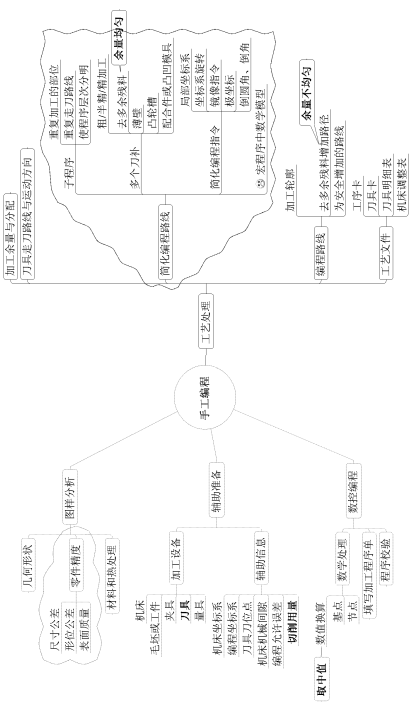
\includegraphics{images/图片1} 
	\caption{手工编程思维导图}\label{手工编程思维导图}
\end{figure}

\subsubsection{数控机床的操作}
如下面的思维导图 \ref{数控机床的操作思维导}
\begin{figure}	
	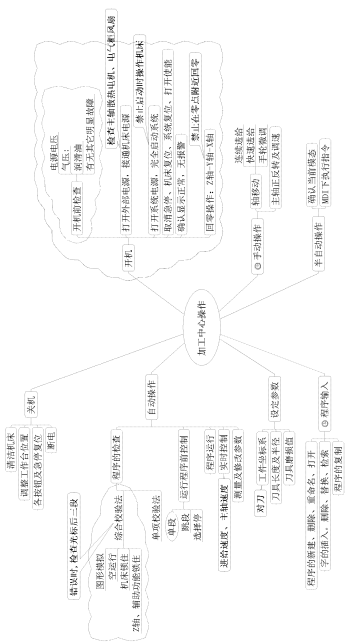
\includegraphics{images/图片2} 
	\caption{数控机床的操作思维导图} \label{数控机床的操作思维导}
\end{figure}

\subsubsection{数控机床指令}
\paragraph{G指令}\begin{itemize}
	\item G0 G1 G2 G3

	\item G17 G18 G19

	\item G9 G61 G62 G63 G64

	\item G4 \marginpar{说明介绍说明介绍说明介绍说明介绍说明介绍说明介绍}

	\item G20 G21

	\item G40 G41 G42 

	\item G43 G44 G49 \marginpar{说明介绍说明介绍说明介绍说明介绍说明介绍说明介绍}

	\item G90 G91

	\item G98 G99

	\item G81 G82 G83 G84 G85 G86 G87 G88 G89 G80 G73 G74 G76

\end{itemize}

\paragraph{M指令}

\begin{itemize}
	\item M0 M1 M2 M30

	\item M3 M4 M5 M19 

	\item M6 M7 M8 M9

	\item M98 M99

\end{itemize}

\paragraph{其它指令}
\subsubsection{常见加工结构}
\begin{itemize}
	\item 平面

	\item 外轮廓

	\item (岛屿)

	\item 孔
	\item 凸轮槽

	\item 复杂零件

	\item 配合零件

	\item CAD/CAM

	\item 宏程序

	\item 其它
\end{itemize}
\subsubsection{上学期期末试卷分析}
\subsection{课堂小结}
主要复习了数控方面的基本知识。
\vfill
\subsection{布置作业}
\begin{enumerate}[1、]
	\item 自选一零件图, 写出其工艺与程序;

	\item 写出如图所示零件的程序及与工艺;
\end{enumerate}
\vfill
